\begin{figure}[H]
\centering
	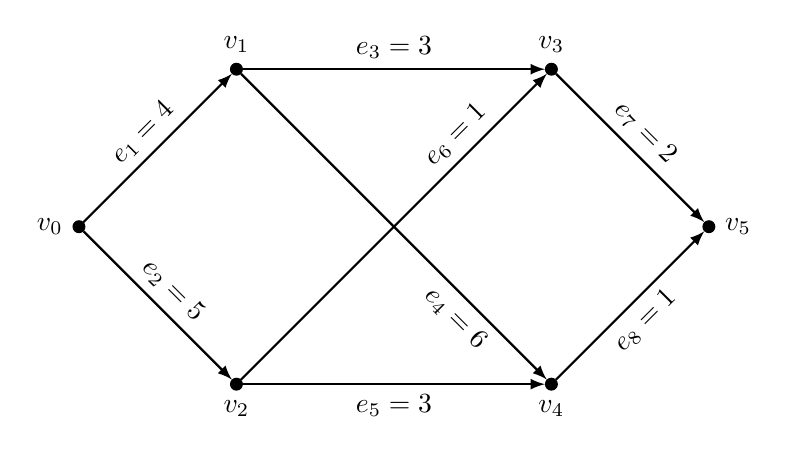
\begin{tikzpicture}

      \tikzset{enclosed/.style={draw, circle, inner sep=0pt, minimum size=.15cm, fill=black}}
%% Vertices
      	\node[enclosed, label={left: $v_0$}] (v0) at (0,2) {};
      	\node[enclosed, label={above: $v_1$}] (v1) at (2,4) {};
    	\node[enclosed, label={below: $v_2$}] (v2) at (2,0) {};
  	    \node[enclosed, label={above: $v_3$}] (v3) at (6,4) {};
     	\node[enclosed, label={below: $v_4$}] (v4) at (6,0) {};
     	\node[enclosed, label={right: $v_5$}] (v5) at (8,2) {};
%Edges
		\path [->, > = latex, thick] (v0) edge node[midway, sloped, above] {$e_1=4$} (v1);
		\path [->, > = latex, thick] (v0) edge node[midway, sloped, above] {$e_2=5$} (v2);
		\path [->, > = latex, thick] (v1) edge node[midway, above] {$e_3=3$} (v3);
		\path [->, > = latex, thick] (v1) edge node[near end, sloped, below] {$e_4=6$} (v4);
		\path [->, > = latex, thick] (v2) edge node[midway, below] {$e_5=3$} (v4);
		\path [->, > = latex, thick] (v2) edge node[near end, sloped, above] {$e_6=1$} (v3);
		\path [->, > = latex, thick] (v3) edge node[midway, sloped, above] {$e_7=2$} (v5);
		\path [->, > = latex, thick] (v4) edge node[midway, sloped, below] {$e_8=1$} (v5);

	\end{tikzpicture}
	\caption{En simpel, orienteret og vægtet graf}
	\label{fig.vaegtetopg}
\end{figure}

